\chapter{Pattern Learning}

\section{Introduction}

Here in pattern learning, we extract the common pattern from a set of ARGs, and the extracted information can then be used to summarize the given ARGs and predict if a new ARG contains the common pattern we summarized. In our work, for instance, we can extract the common structure of a set of proteins that share the same function. The common structure we extracted can give us insight on how this structure can perform such function, and if a new protein also has the same structure that can carry out the same function.\\

To perform pattern learning, we utilize a probabilistic parametric model to represent the common pattern from the graphs (Hong\footnotemark and Huang 2004). Similar to how three normal distribution (or components) can capture the data distribution generated by $f(x)$ below, we used a couple component ARGs with various mean and variance to represent the common pattern:
\footnotetext{My dear advisor!}

\begin{figure}[h]
	\centering
	\captionsetup{justification=centering}
	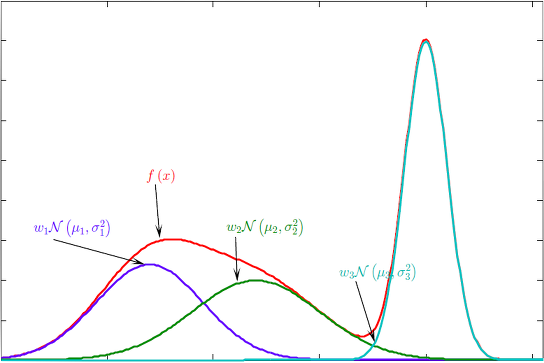
\includegraphics[width=0.65\textwidth]{figs/mixture.png}
	\caption[Caption for LOF]{\emph{The data distribution generated by $f(x)$ can be captured by three normal distribution with various means and variances.}}
	\label{fig:mixture}
\end{figure}

Therefore, the model training process is essentially training and setting up some component ARGs so that all the nodes and edges have the means and variances that best capture the common pattern in the given set of ARGs.\\

Based on the algorithm described by Hong and Huang, we first pick some ARGs from the input sample ARGs, and initialize them as the component ARGs. Then we perform an EM algorithm where on the \textbf{E}xpectation step we run the graph matching algorithm to calculate the matching probability between model ARGs and sample ARGs while on the \textbf{M}aximization step we update the model ARG (e.g. updating means, variances, and deleting redundant nodes) in order to achieve higher matching probability. Finally, once the update is very small, we output the model ARGs to represent the common pattern in sample ARGs:

\begin{figure}[h]
	\centering
	\captionsetup{justification=centering}
	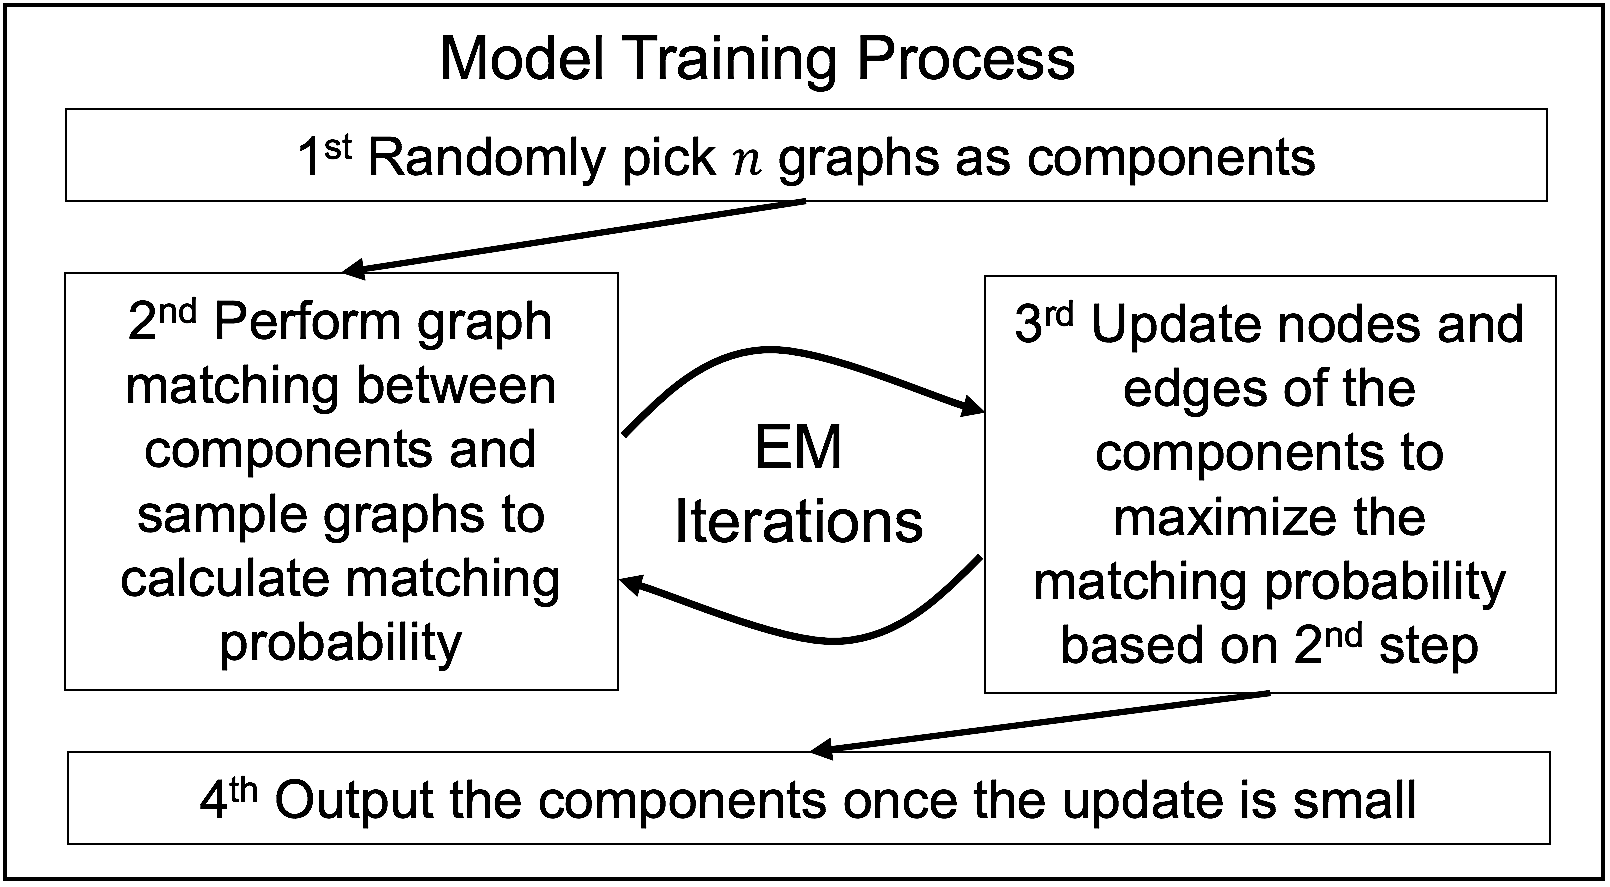
\includegraphics[width=0.7\textwidth]{figs/model_training.png}
	\caption[Caption for LOF]{\emph{The probabilistic parametric model training process with EM algorithm.}}
	\label{fig:model_training}
\end{figure}

\section{Syntax and Definition}

The sample ARGs (i.e. the set of ARGs we want to learn/extract pattern from) is denoted as $\{G_s\}_{s=1}^S$ where $S$ is the number of model components. Within each sample ARG, we indicate the label for each node and edge as $N^s_a$ and $E^s_{ab}$. This is similar to what we have in Chapter 1 but with an additional index $s$ indicating which sample these nodes and edges belong to.\\

For the model, we denoted it as $Z$ and the model consists of a set of parametric model components $\{\Phi_w\}_{w=1}^W$ where $W$ is the number of model components. For each component, there are also an associated weight $\alpha_w$ which indicates how much information the component captures and how important the component is.\\

Within each component ARG, we indicate the mean for each node and edge as $N^w_a$ and $E^w_{ab}$ similar to what we have for sample ARGs, but with $w$ instead of $s$ indicating which model this node and edge belongs to. In addition to the mean, there are also the covariance matrixes for node and edge denoted by $\Sigma^w_a$ and $\Sigma^w_{ab}$ with a similar index. Last but not least, for each node in each component, there is an associated frequency/weight $\beta^w_a$ indicating how important one node is and if we can delete such node.\\